\begin{figure}[!htb]
\begin{minipage}{0.5\textwidth}  
\begin{tikzpicture}[remember picture,baseline=0]
%%
  \node (G) {
   
   \begin{tikzpicture}[main node/.style={circle,draw,minimum size=.8cm,inner sep=0pt}]
  	
	 \path   (0, 0)  node[main node]  (2) {$a$}
	         (2, 0)  node[main node]  (3) {$b$}
	         (1, -2)  node[main node] (4) {$c$}
	         (0, -4)  node[main node] (5) {$d$}
			 (2, -4)  node[main node] (6) {$e$}
			 (1, -6)  node[main node] (7) {$f$}
			 (-1, -2)  node[main node] (8) {$g$};

	\path[->, thick]
			(2) edge node {} (4)
			(2) edge node {} (8)
			(8) edge node {} (5)
			(3) edge node {} (4)
			(4) edge node {} (5)
			(4) edge node {} (6)
			(5) edge node {} (7)
			(6) edge[bend right] node {} (4)
			(6) edge node {} (7);
		
	\draw[->, dashed] (0,1) to node {} (2);
	\draw[->, dashed] (2,1) to node {} (3);
	\draw[->, dashed] (7) to node {} (0, -7);
	\draw[->, dashed] (7) to node {} (2, -7);

    \draw (0,-8) node {$G$};
  	\end{tikzpicture}
  };

    %%
    \node(H)[right=of G]{
	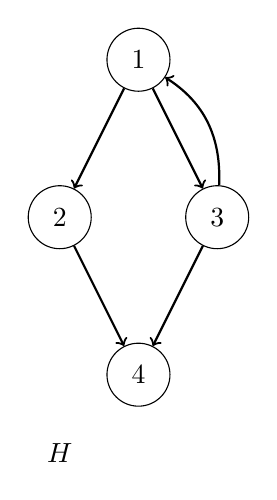
\begin{tikzpicture}[main node/.style={circle,draw,minimum size=.8cm,inner sep=0pt}]
  	 \path   (1, -2)  node[main node] (4) {$1$}
  	         (0, -4)  node[main node] (5) {$2$}
  			 (2, -4)  node[main node] (6) {$3$}
  			 (1, -6)  node[main node] (7) {$4$};
  
  	\path[->, thick]
  			(4) edge node {} (5)
  			(4) edge node {} (6)
  			(5) edge node {} (7)
  			(6) edge[bend right] node {} (4)
  			(6) edge node {} (7);
    \draw (0,-7) node {$H$};
    \end{tikzpicture}   
    };
\end{tikzpicture}
\end{minipage}\hfill
\begin{minipage}{0.5\textwidth}
Let $H=(V',E')$ and $G=(V,E)$ then a possible assignments is a function $P: V' \to V''$
\begin{itemize}
\item $P(1) =\{c, e, f,\dots\} $
\item $P(2) =\{a, b, c, d, g,\dots \} $
\item $P(3) =\{c, e,\dots\} $
\item $P(4) =\{c, f,\dots\} $
\end{itemize}
\end{minipage}
\caption{Possible assignments for a subgraph.}
\label{fig:possibleassignment_example}
\end{figure}